%\documentclass[12pt, twoside]{book}
\documentclass[12pt, oneside]{book}  % jednostranna tlac

%spravne nastavenie okrajov
\usepackage[a4paper,top=2.5cm,bottom=2.5cm,left=3.5cm,right=2cm]{geometry}
%zapnutie fontov pre UTF8 kodovanie
\usepackage[utf8]{inputenc}
\usepackage[T1]{fontenc}
\usepackage{lmodern}

%zapnutie slovenskeho delenia slov
%a automatickych nadpisov ako Obsah, Obrázok a pod. v slovencine
\usepackage[slovak]{babel} % vypnite pre prace v anglictine!

%nastavenie riadkovania podla smernice
\linespread{1.25} % hodnota 1.25 by mala zodpovedat 1.5 riadkovaniu

% balicek na vkladanie zdrojoveho kodu
\usepackage{listings}
% ukazky kodu su cislovane ako Listing 1,2,...
% tu je Listing zmenene na Algoritmus 1,2,...
\renewcommand{\lstlistingname}{Algoritmus}
% nastavenia balicka listings
% mozete pridat aj language=...
% na nastavenie najcastejsie pouzivaneho prog. jazyka
% takisto sa da zapnut cislovanie riadkov
\lstset{frame=lines,language=Java}
% balicek na vkladanie obrazkov
\usepackage{graphicx}
% balicek na vkladanie celych pdf dokumentov, tu zadanie
\usepackage{pdfpages}
% balicek na spravne formatovanie URL
\usepackage{url}
% balicek na hyperlinky v ramci dokumentu
% zrusime farebne ramiky okolo liniek aby pdf
% vyzeralo rovnako ako tlacena verzia
\usepackage[hidelinks,breaklinks]{hyperref}
\usepackage{amssymb}
\usepackage{amsmath}
\newcommand{\Lang}{\mathcal{L}}
\newcommand{\Struct}{\mathcal{M}}
\newcommand{\Vars}{\mathcal{V}_\Lang}
\newcommand{\Funcs}{\mathcal{F}_\Lang}
\newcommand{\Preds}{\mathcal{P}_\Lang}
\newcommand{\Consts}{\mathcal{C}_\Lang}
\newcommand{\Terms}{\mathcal{T}_\Lang}
\newcommand{\Atoms}{\mathcal{A}_\Lang}
\newcommand{\Forms}{\mathcal{E}_\Lang}

% -------------------
% --- Definicia zakladnych pojmov
% --- Vyplnte podla vasho zadania, rok ma byt rok odovzdania
% -------------------
\def\mfrok{2026}
\def\mfnazov{Kontrola ekvivalentných úprav v interaktívnom logickom pracovnom zošite}
\def\mftyp{Bakalárska práca}
\def\mfautor{Jakub Šimon Štofanik}
\def\mfskolitel{Mgr. Ján Kľuka, PhD.}

%ak mate konzultanta, odkomentujte aj jeho meno na titulnom liste
%\def\mfkonzultant{tit. Meno Priezvisko, tit. }  

\def\mfmiesto{Bratislava, \mfrok}

% študenti BIN a DAV odkomentujú príslušnú dvojicu riadkov
\def\mfodbor{ Informatika}
\def\program{ Aplikovaná Informatika }

% Ak je školiteľ z FMFI, uvádzate katedru školiteľa, zrejme by mala byť aj na zadaní z AIS2
% Ak máte externého školiteľa, uvádzajte Katedru informatiky 
\def\mfpracovisko{ Katedra informatiky }

\begin{document}     
\frontmatter
\pagestyle{empty}

% -------------------
% --- Obalka ------
% -------------------

\begin{center}
\sc\large
Univerzita Komenského v Bratislave\\
Fakulta matematiky, fyziky a informatiky

\vfill

{\LARGE\mfnazov}\\
\mftyp
\end{center}

\vfill

{\sc\large 
\noindent \mfrok \hfill
\mfautor
}

\cleardoublepage
% --- koniec obalky ----

% -------------------
% --- Titulný list
% -------------------


\noindent

\begin{center}
\sc  
\large
Univerzita Komenského v Bratislave\\
Fakulta matematiky, fyziky a informatiky

\vfill

{\LARGE\mfnazov}\\
\mftyp
\end{center}

\vfill

\noindent
\begin{tabular}{ll}
Študijný program: & \program \\
Študijný odbor: & \mfodbor \\
Školiace pracovisko: & \mfpracovisko \\
Školiteľ: & \mfskolitel \\
% Konzultant: & \mfkonzultant \\
\end{tabular}

\vfill


\noindent \mfmiesto \hfill
\mfautor

\cleardoublepage
% --- Koniec titulnej strany


% -------------------
% --- Zadanie z AIS
% -------------------
% v tlačenej verzii s podpismi zainteresovaných osôb.
% v elektronickej verzii sa zverejňuje zadanie bez podpisov
% v pracach v angličtine anglické aj slovenské zadanie

\newpage 
\setcounter{page}{2}
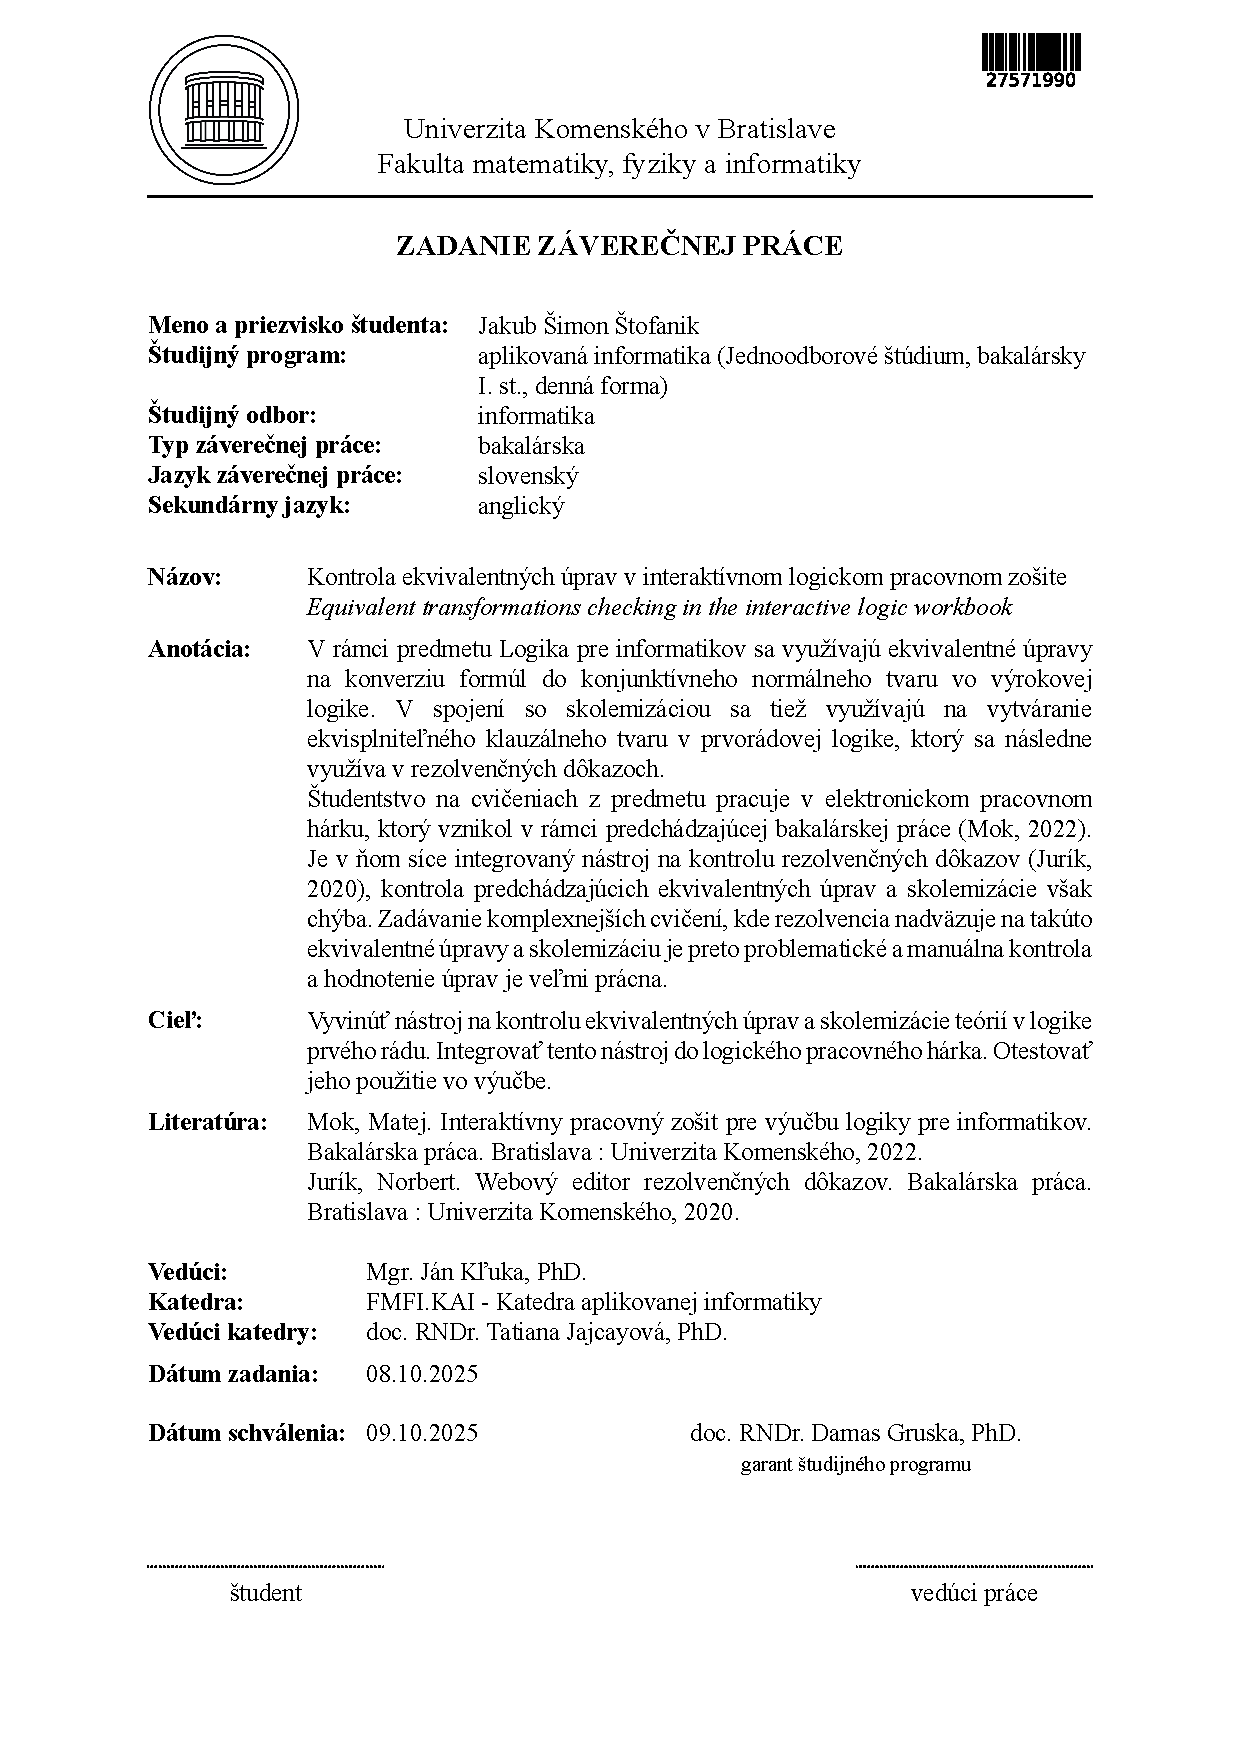
\includepdf{images/zadanie.pdf}

% --- Koniec zadania


% -------------------
%   Abstrakt - Slovensky
% -------------------
\newpage 
\section*{Abstrakt}

V tejto práci sa venujeme vývoju webovej aplikácie, ktorá bude použitá ako učebná pomôcka. Aplikácia je určená na kontrolu ekvivalentných úprav logických formúl a skolemizácie, pomocou ktorých sa logické formuly prevádzajú do konjunktívnej normálnej formy. Pomocou prvorádového jazyka zadaného používateľom aplikácia skontroluje správnosť úprav formúl. Aplikácia bude kontrolovať iba samotné ekvivalentné úpravy a skolemizáciu, samotný postup je ponechaný na používateľa. Na vývoj aplikácie boli použité knižnice React a Redux. Aplikácia bude použitá ako učebná pomôcka pri výučbe predmetu Logika pre informatikov a bude integrovaná do interaktívneho logického zošita, ktorý sa na predmete využíva. Aplikácia bola úspešne testovaná v rámci spomenutého predmetu počas letného semestra 2025/2026.
%Slovenský abstrakt v rozsahu 100-500 slov, jeden odstavec. Abstrakt
%stručne sumarizuje výsledky práce. Mal by byť pochopiteľný pre bežného
%informatika. Nemal by teda využívať skratky, termíny alebo označenie
%zavedené v práci, okrem tých, ktoré sú všeobecne známe.

\paragraph*{Kľúčové slová:} logika prvého rádu, Logic Workbook, prevod do konjunktívnej normálnej formy, CNF, webová aplikácia %jedno, druhé, tretie (prípadne štvrté, piate)
% --- Koniec Abstrakt - Slovensky


% -------------------
% --- Abstrakt - Anglicky 
% -------------------
\newpage 
\section*{Abstract}

In this work, we are developing a web application that will be used as a teaching aid. The application is designed to check equivalent transformations of logical formulas and skolemization, with which logical formulas are converted to conjunctive normal form. Using the language of first-order logic entered by the user, the application will check the correctness of the formula transformations. The application will only check the equivalent transformations and skolemization themselves, the conversion to conjunctive normal form is left to the user. The React and Redux libraries were used to develop the application. The application will be used as a teaching aid in the teaching of the subject Logic for Computer Scientists and will be integrated into the interactive Logic Workbook that is used during the subject. The application was successfully tested within the aforementioned subject during the summer semester 2025/2026.

\paragraph*{Keywords:} first order logic, Logic Workbook, conversion to conjunctive normal form, CNF, web application

% --- Koniec Abstrakt - Anglicky

% -------------------
% --- Predhovor - v informatike sa zvacsa nepouziva
% -------------------
%\newpage 
%
%\chapter*{Predhovor}
%
%Predhovor je všeobecná informácia o práci, obsahuje hlavnú charakteristiku práce 
%a okolnosti jej vzniku. Autor zdôvodní výber témy, stručne informuje o cieľoch 
%a význame práce, spomenie domáci a zahraničný kontext, komu je práca určená, 
%použité metódy, stav poznania; autor stručne charakterizuje svoj prístup a svoje 
%hľadisko. 
%
% --- Koniec Predhovor


% -------------------
% --- Obsah
% -------------------

\newpage 

\tableofcontents

% ---  Koniec Obsahu

% -------------------
% --- Zoznamy tabuliek, obrázkov - nepovinne
% -------------------

\newpage 

\listoffigures
%\listoftables

% ---  Koniec Zoznamov

\mainmatter
\pagestyle{headings}


\input uvod.tex 

\input teoretickeZnalosti.tex 

\input vychodisko.tex 


\input navrh.tex 

\input implementacia.tex 


\input testovanie.tex 

\input zaver.tex

% -------------------
% --- Bibliografia
% -------------------


\newpage	

\backmatter

\thispagestyle{empty}
\clearpage

\bibliographystyle{plain}
\bibliography{literatura} 


\input appendixA.tex


























\end{document}







